\documentclass[]{article}
\usepackage[margin=2cm]{geometry}

%opening
\title{Exercises Set: Optimization}
\author{DSBA Mathematics Refresher 2025}
\date{}

\usepackage{amsmath}
\usepackage{amsfonts}
\usepackage{amsthm}
\usepackage{amssymb}
\usepackage{mathrsfs}
\usepackage{stmaryrd}
\usepackage{tikz}

\newcommand{\Q}{\mathbb{Q}}
\newcommand{\N}{\mathbb{N}}
\newcommand{\Z}{\mathbb{Z}}
\newcommand{\R}{\mathbb{R}}
\newcommand{\Primes}{\mathbb{P}}
\newcommand{\st}{\text{ s.t. }}
\newcommand{\txtand}{\text{ and }}
\newcommand{\txtor}{\text{ or }}
\newcommand{\lxor}{\veebar}


\begin{document}
	
	\maketitle
	
	\begin{abstract}
		Only the questions with a * are compulsory (but do all of them!).
	\end{abstract}
	
	\section{Optimization}
	\subsection{One dimension}
	Let's consider $f(x) = x^2-x+3$.
	We are interested in finding the minimum of this function; 
	i.e. we want to find $x^* \in \R$ such that $f(x^*)$ is the smallest possible, mathematically:
	$$\forall x\in \R, f(x) \geq f(x^*)$$
	\textit{It turns out that since this function is quadratic, you can manually compute that $x^*=0.5$.
		However, we will suppose that this is a complex function, for which we cannot find the minimum by hand.
		The techniques we will develop should be generalization to more complex functions, for which you won't be able to find the minimum "by hand".}
	
	\paragraph{Method 1}
	First, let's try to brute force our problem: compute $f(x)$ for $x=-1.75$, $x=-1.25$, $x=-0.75$, $x=-0.25$, $x=0.25$, $x=0.75$, $x=1.25$, $x=1.75$, $x=2.25$, $x=2.75$, and $x=3.25$.\\
	Find the $x$ value that gave you the smallest value for $f(x)$.
	This will be you first "guess" for $x^*$.\\
	\begin{center}
		\begin{tikzpicture}[xscale=1.05,yscale=0.30]
			\draw[->] (-2.5,0) -- (3.9,0) node[right] {\scriptsize $x$};
			\draw[->] (0,0) -- (0,11.5) node[above] {\scriptsize $f(x)$};
			\foreach \t in {5,10}{ \draw (0.06,\t) -- (-0.06,\t) node[left] {\scriptsize $\t$}; }
			\draw[thick,domain=-2.2:3.4,samples=80,smooth] plot ({\x},{\x*\x-\x+3});
			\foreach \p in {-1.75,-1.25,-0.75,-0.25,0.25,0.75,1.25,1.75,2.25,2.75,3.25}{
				\draw[dotted,gray] ({\p},0) -- ({\p},{\p*\p-\p+3});
				\node[circle,fill,minimum size=3.2pt,inner sep=0] at ({\p},{\p*\p-\p+3}) {};
			}
		\end{tikzpicture}
	\end{center}
	\textbf{This technique is called "grid search".}\\
	List the positive and negative aspect of this technique.
	
	\paragraph{Method 2}
	For this second approach, we will suppose that $x^*$ is in $(-5,5)$.\\
	Define $a=-5$ and $b=5$, and iterate the following process:
	\begin{itemize}
		\item if $f(a)>f(b)$, then let $a = \frac{a+b}{2}$
		\item if $f(a)<f(b)$, then let $b = \frac{a+b}{2}$
	\end{itemize}
	Manually do 6-7 steps of this process.
	Your final "guess" for $x^*$ is $\frac{a+b}{2}$.\\
	\textbf{This technique is called "dichotomy".}\\
	List the positive and negative aspect of this technique.
	
	\paragraph{Method 3}
	For this second approach, we will suppose that $x^*$ is "close" to\footnote{or at least "not too far" from} $-0.5$.\\
	Define $x_0=-0.5$, choose a 'learning rate' $\lambda=0.8$ (say) and iterate the following process:
	\begin{itemize}
		\item compute $f'(x_k)$
		\item let $x_{k+1} = x_k - \lambda * f'(x_k)$
	\end{itemize}
	(*) Manually do 5 steps of this process.
	Your final "guess" for $x^*$ is the last $x_k$ calculated.\\
	Repeat the process with $\lambda=0.3$, $\lambda=0.1$, $\lambda=1$, $\lambda=2$. (calculators / computers are allowed!)\\
	Give some conclusion on how to choose $\lambda$.\\
	\begin{center}
		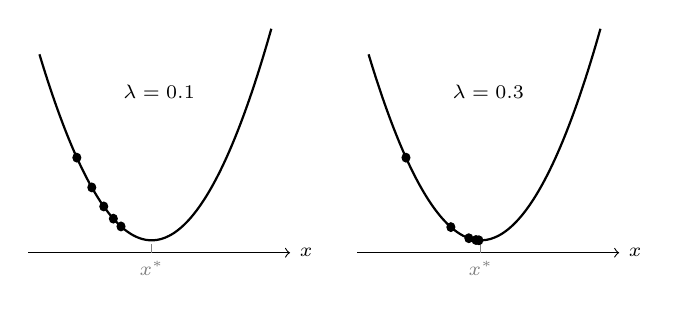
\begin{tikzpicture}[xscale=0.95,yscale=1.05]
			\foreach \dx/\lab/\pts in {%
				0/{$\lambda=0.1$}/{-0.5,-0.3,-0.14,-0.012,0.0904},
				4.4/{$\lambda=0.3$}/{-0.5,0.1,0.34,0.436,0.4744}}{
				\begin{scope}[xshift=\dx cm]
					\draw[->] (-1.15,2.6) -- (2.35,2.6) node[right] {\scriptsize $x$};
					\draw[thick,domain=-1.0:2.1,samples=60,smooth] plot ({\x},{\x*\x-\x+3});
					\draw[dashed,gray] (0.5,2.6) -- (0.5,2.75);
					\node[gray,below] at (0.5,2.62) {\scriptsize $x^*$};
					\foreach \p in \pts { \filldraw ({\p},{\p*\p-\p+3}) circle (1.5pt); }
					\node at (0.6,4.55) {\scriptsize \lab};
				\end{scope}
			}
		\end{tikzpicture}\\[2mm]
		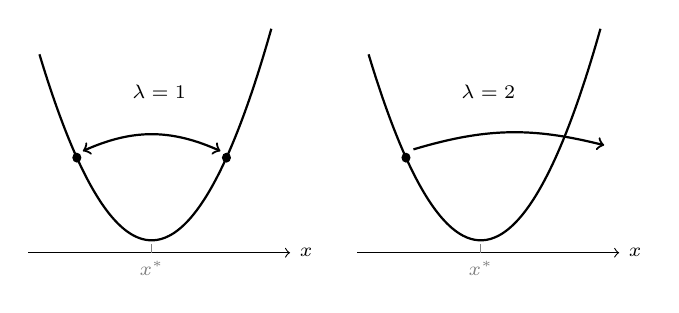
\begin{tikzpicture}[xscale=0.95,yscale=1.05]
			\begin{scope}
				\draw[->] (-1.15,2.6) -- (2.35,2.6) node[right] {\scriptsize $x$};
				\draw[thick,domain=-1.0:2.1,samples=60,smooth] plot ({\x},{\x*\x-\x+3});
				\draw[dashed,gray] (0.5,2.6) -- (0.5,2.75);
				\node[gray,below] at (0.5,2.62) {\scriptsize $x^*$};
				\filldraw (-0.5,3.75) circle (1.5pt);
				\filldraw (1.5,3.75) circle (1.5pt);
				\draw[<->,thick] (-0.42,3.83) to[bend left=22] (1.42,3.83);
				\node at (0.6,4.55) {\scriptsize $\lambda=1$};
			\end{scope}
			\begin{scope}[xshift=4.4cm]
				\draw[->] (-1.15,2.6) -- (2.35,2.6) node[right] {\scriptsize $x$};
				\draw[thick,domain=-1.0:2.1,samples=60,smooth] plot ({\x},{\x*\x-\x+3});
				\draw[dashed,gray] (0.5,2.6) -- (0.5,2.75);
				\node[gray,below] at (0.5,2.62) {\scriptsize $x^*$};
				\filldraw (-0.5,3.75) circle (1.5pt);
				\draw[->,thick] (-0.4,3.85) to[bend left=14] (2.15,3.9);
				\node at (0.6,4.55) {\scriptsize $\lambda=2$};
			\end{scope}
		\end{tikzpicture}
	\end{center}
	\textit{(the dots are the successive $x_k$; $x^*$ marks the true minimum)}\\
	\textbf{This technique is called "gradient descent".}\\
	List the positive and negative aspect of this technique.
	
	\subsection{Two dimensions}
	Let's consider $f(x,y) = (x+y-1)^2 + \frac{1}{5}(x-y)^2$.
	We are interested in finding the minimum of this function; 
	i.e. we want to find $(x^*,y^*) \in \R^2$ such that $f(x^*,y^*)$ is the smallest possible, mathematically:
	$$\forall (x,y) \in \R^2, f(x,y) \geq f(x^*, y^*)$$
	\textit{Again, it is possible to manually compute that the minimum is reached for $(x^*, y^*) = (0.5, 0.5)$; however, we suppose that we do not know this.}
	
	Generalize the three methods used in 1D to apply them in 2D.
		
	Explain how the computational cost evolve for each technique as the number of dimensions increases.
	
	\section{Regression}
	(*) With justification, find \textbf{the} line of best fit of the following points:
	\begin{itemize}
		\item $P_1 = (0,1)$
		\item $P_2 = (3,8)$
		\item $P_4 = (5,12)$
		\item $P_5 = (8,17)$
	\end{itemize}
	\begin{center}
		\begin{tikzpicture}[xscale=0.48,yscale=0.25]
			\draw[->] (-0.6,0) -- (9.6,0) node[right] {\scriptsize $x$};
			\draw[->] (0,-0.8) -- (0,20.5) node[above] {\scriptsize $y$};
			\foreach \t in {2,4,6,8}{ \draw (\t,0.4) -- (\t,-0.4) node[below] {\scriptsize $\t$}; }
			\foreach \t in {5,10,15}{ \draw (0.12,\t) -- (-0.12,\t) node[left] {\scriptsize $\t$}; }
			\draw[gray,thick] (-0.3,3.4) -- (9.3,16.36);
			\node[gray,below right] at (7.3,13.7) {\scriptsize a candidate line};
			\foreach \px/\py in {0/1,3/8,5/12,8/17}{
				\draw[dashed,red,thick] ({\px},{\py}) -- ({\px},{1.35*\px+3.8});
				\node[circle,fill,minimum size=4.4pt,inner sep=0] at ({\px},{\py}) {};
			}
			\node[red,left] at (4.85,11.2) {\scriptsize error};
		\end{tikzpicture}
	\end{center}
	\textit{Which line makes the (dashed) errors as small as possible, and in what sense?}
	
	
\end{document}
